\section{Covariance estimation}
The LIMIX framework enables multi-trait LMM analyses for more than two traits and provides methods to decompose phenotypic variance \citep{Lippert2014}. In single-variant LMMs, typically two phenotypic variance components are assumed: i) a genetic component \(g\) and ii) a noise component \(\psi\) (Equations \ref{eq:lmm-uv} and \ref{eq:lmm-mv}). 
\noindent To estimate the variance decomposition (VD) into \(g\) and \(\psi\), the phenotype is described as the null model of the LMM:
\begin{equation}
\mathbf{y} = \mathbf{g}+\boldsymbol{\psi},\text{ }
\mathbf{g}\sim
\mathcal{N}\left(0,
\mathbf{C_g} \otimes \mathbf{R}\right),\text{ }
 \mathbf{\psi}\sim
\mathcal{N}\left(0,\mathbf{C_n} \otimes \mathbf{I_n}\right)
\label{eq:vd}
\end{equation}



The sample-by-sample covariances of the genetic and noise term, \(R\) and \(I_N\), are provided and the model estimates the trait-by-trait covariance matrices \(C_g\) and \(C_n\). The complexity of the VD is \(O(N^2 + t(NP^2 + NP^4))\) with \(N\) the number of samples, \(P\) the number of traits, and \(t\) the number of iterations of Broyden's method for optimising the restricted marginal likelihood (RML) of the parameter estimates. From this equation, it becomes evident that as the number of traits increases, the complexity increases by a power of four and explains why the LMM is not feasable for large trait sets. In order to to allow for multi-trait mapping of large trait sets, a bootstrapping-based approach was investigated. Instead of modeling all traits at the same time, a subset of \(s\) traits is randomly selected, the VD computed  and the $s \times s$ covariance matrices $C^*_g$ and $C^*_n$ recorded. This random selection with replacement is repeated \(n\) times such that each two traits are drawn together at least ten times, with \(n\) depending on the overall trait size \(P\) and the sampling size \(s\).  The challenge after the VD is to combine the bootstrap results in a way, that the resulting $C_g$ and $C_n$ are true covariance matrices, i.e. positive semi-definite matrices. Simply averaging values over all bootstrapping results leads to matrices with negative eigenvalues which have to be regularized to achieve positive semi-definiteness. The regularization leads to an overestimation of the trait variances (diagonal) compared to the trait-trait covariances (off-diagonal). In order to circumvent this overestimation, the unregularized averaged $C_g$ and $C_n$ are used as an initial guess to fit a residual sum of squares model over all bootstrap runs. The model makes use of cholesky decomposition of the matrix to be fitted, resulting in $\frac{1}{2}P(P+1)$ model parameters to be fitted. The fitting is achieved by using the BFGS optimizer, a limited memory quasi-Newton algorithm for solving large nonlinear optimization problems \citep{Byrd1995}.  $C_g$ and $C_n$ are fitted separately. The complexity of LiMMBo is \(O(N^2 + nt_1(Ns^2 + Ns^4) + t_2(\frac{1}{2}P(P+1))\), which is the sum of the complexity of the VD as described above for the subset of \(s\) traits and the complexity of fitting the BFGS algorithm \(t_2\) times for the full trait set size \(P\). 


\section{Simulated dataset}
\label{section:simulateddata}
In order to assess calibration and power of LiMMBo, genotypes and phenotypes were simulated similar to strategies described in \citep{Loh2014,Casale2015}.  
\paragraph{Genotypes.} \label{paragraph:genotypes}
The synthetic genotypes were generated based on real genotype data from four European ancestry populations of the 1000 Genomes (1KG) Project (populations: CEU, FIN, GBR, TSI) \citep{Abecasis2012}. Depending on the cohort structure, each newly synthesised individual is assigned to \(N\) ancestors from the original 1KG Project and their genome split into blocks of 1,000 SNPs (thereby retaining realistic LD structure between SNPs). For each SNP block, an ancestor is chosen at random and its genotype is copied to the individuals genome. Low numbers of \(N\) introduce relatedness among indivduals, whereas high numbers of \(N\) lead to low levels of structure and relatedness. By allowing random selection of the ancestors from the four subpopulations, population structure will be low, whereas predefining subpopulation of the ancestor can give rise to structured populations. Three distinct cohorts of 1,000 individuals each were generated: i) unrelated individuals, with population structure (unrelatedPopStructure): \(N=10\), prior assigment to ancestorial population , ii) unrelated individuals, no population structure (unrelatedNoPopStructure): \(N=10\), no prior assigment to ancestorial population and iii) related individuals, no population structure (relatedNoPopStructure): \(N=2\), no prior assigment to ancestorial population.  The genetic relatedness matrices and scatter plots of the first two principal components for each cohort are shown in Figure~\ref{fig:kinship-matrices}. 


\begin{figure}[!h]
	\centering
	\includegraphics[page=2, trim = 0mm 10mm 15mm 0mm, clip, scale=0.25]{Chapter1/Figures/20170131_simulatedCovarianceMatrices_kinship.png}
	\caption[Kinship matrices and principle components of three simulated European ancestry cohorts]{\textbf{Kinship matrices and principle components of three simulated European ancestry cohorts.} The genotypes were simulated based in genotype data from four Europen ancestry population (ancestry color key in panel a). Depending on the choice and number of ancestors for the sampling of chromosomes to simulate an individulas genotype, cohorts with differing levels of population and relatedness structure will arise. (a) unrelated individuals, with population structure: \(N=10\), prior assigment to ancestorial population. (b) unrelated individuals, no population structure: \(N=10\), no prior assigment to ancestorial population. (c) related individuals, no population structure: \(N=2\), no prior assigment to ancestorial population.}
 	\label{fig:kinship-matrices}
\end{figure}


\paragraph{Phenotypes.} The phenotypes \( \mat{Y} \in \mathcal{R}^{N,P}\) of \(N\) samples and \(P\) traits were generated as the sum of four components: i) fixed genetic effects \( \mat{U} \in \mathcal{R}^{N,P}\) , ii) random genetic effects \( \mat{G} \in \mathcal{R}^{N,P}\), iii) fixed noise effects\( \mat{C} \in \mathcal{R}^{N,P}\) and iv) random noise effects \( \mat{\Psi} \in \mathcal{R}^{N,P}\). For each component, a certain percentage of variance is shared across all traits (\textit{shared}) and the remainder is independent (\textit{ind}) across traits.

\begin{enumerate}
\item \textit{Fixed genetic effects \tmat{U}}. For the fixed genetic effects,  \(S\) random SNPs for \(N\) samples were drawn from the simulated genotypes. From the \(S\) random SNPs, a proportion \tbm{\theta} was selected to be causal across all traits. \(\mat{U}^{shared} \in \mathcal{R}^{N,P}\) was simulated as the matrix product of this shared causal SNP matrix \(\mat{X}^{shared} \in \mathcal{R}^{N,\theta  \text{x} S}\) and a \(\mat{B}^{shared} \in \mathcal{R}^{\theta  \text{x} S, P}\) shared effect size matrix. \(\mat{B}^{shared}\) in turn is the matrix product of the two normally distributed vectors \(b_s \in \mathcal{R}^{\theta  \text{x} S,1}\) and \(b_p^T \in \mathcal{R}^{1,P}\). The remaining \((1- \theta ) \text{x} S\) SNPs were simulated to have an idependent effect across a limited number of traits \(p^{ind}\). To realise this structure, \(\mat{B}^{ind}  \in \mathcal{R}^{(1-\theta)  \text{x} S, P}\) is initialised with normally distributed entries. Subsequently, \(1 - p^{ind}\) traits are randomly selected and the row entries for \(\mat{B}^{ind}\) at these traits set to zero. \(\mat{U}^{ind} \in \mathcal{R}^{N,P}\) is the matrix product of  \(\mat{X}^{ind} \in \mathcal{R}^{N,(1 - \theta)  \text{x} S}\)  and \(\mat{B}^{ind}\).
The fixed genetic effect \tmat{U} is the sum of \(\mat{U}^{shared}\) and \(\mat{U}^{ind}\).

\item \textit{Fixed noise effects \tmat{C}} The fixed noise effects\tmat{C} are based on \(K\) normally distributed confounders \(\mat{F} \in \mathcal{R}^{N,K}\), with a proportion \(\gamma\) being shared across all traits yielding the shared confounder matrix \(\mat{F}^{shared} \in \mathcal{R}^{\gamma  \text{x} K, P}\). The proportion of \(1- \gamma\) confounder that are independent build the independent confounder matrix \(\mat{F}^{ind} \in \mathcal{R}^{(1-\gamma)  \text{x} K, P}\). The effect size matrices  \(\mat{A}^{shared}  \in \mathcal{R}^{(\gamma)  \text{x} K, P}\)  and \(\mat{A}^{ind}  \in \mathcal{R}^{(1-\gamma)  \text{x} K, P}\) were designed in analogy to the ones for the fixed genetic effects. The total fixed noise effect is then \(\mat{C} = \mat{K}^{shared}\mat{A}^{shared} +  \mat{K}^{ind}\mat{A}^{ind}\).

\item \textit{Random genetic effects} The random genetic effects \(\mat{G} \in \mathcal{R}^{N,P}\) are modeled as a matrix-normally distributed random variable, defined by its mean \(\mat{M} \in \mathcal{R}^{N,P}\), its column covariance \(\mat{C} \in \mathcal{C}^{P,P}\) and its row covariance \(\mat{R} \in \mathcal{R}^{N,N}\).  
\begin{equation}
\mat{G} \sim MN_{N,P}(0,\mat{R},\mat{C}) 
\end{equation}

The \(N \text{x} N\) kinship matrix $K$, estimated according to Equation~\ref{eq:kinship} from the SNP genotypes of simulated samples represents \tmat{R}.  The structure of the trait-to-trait covariance \tmat{C} depends on the design ot the effect, shared or independent. To construct \tmat{G}, assume a matrix-normally distributed random variable \tmat{Z} with \(\mat{M}=0\)  and \(\mat{R} = \mat{K}\):

\begin{equation}
\mat{Z} \sim MN_{N,P}(0,\mat{K},\mat{C}) 
\end{equation}

\tmat{Z} can be expressed in terms of a multivariate normal distribution 

\begin{equation}
vec(Z) \sim N_{N\text{x}P}(0, \mat{C} \otimes \mat{K})
\end{equation}

With the cholesky decompositon of \tmat{K} and \tmat{C} into  \(\mat{K}=\mat{BB}^T\) and \(\mat{C}=\mat{AA}^T\) 

\begin{equation}
vec(Z) \sim N_{N\text{x}P}(0, \mat{AA}^T \otimes \mat{BB}^T)
\end{equation}

which can be rearranged  as 

\begin{equation}
\begin{aligned}
vec(\mat{Z}) \sim N(0, (\mat{A} \otimes \mat{B}) I (\mat{A}^T \otimes \mat{B}^T) \\
vec(\mat{Z})  \sim N(0, (\mat{A }\otimes \mat{B}) I (\mat{A} \otimes\mat{B})^T) 
\end{aligned}
\end{equation}

Using the property of 
\begin{equation}
\begin{aligned} 
\mat{Y} \sim N(0, \Sigma) \\
w \mat{Y} \sim N(0, w\Sigma w^T)
\end{aligned}
\end{equation}

we can let  \(vec(\mat{}Z) =  (\mat{A} \otimes \mat{B})vec(\mat{Y})\) such that
\begin{equation}
\begin{aligned}
(\mat{A} \otimes\mat{B})vec(\mat{Y})  \sim N(0, (\mat{A} \otimes \mat{B}) I (\mat{A} \otimes \mat{B})^T) 
\end{aligned}
\end{equation}

Using \citep{Horn1991}: Lemma 4.3.1, we get 
\begin{equation}
(\mat{A} \otimes \mat{B}) vec(\mat{Y}) = vec(\mat{BYA}^T) 
\end{equation}

For the independent effect, \(\mat{A}^{ind}\) is a diagonal matrix with normally distributed entries: \(\mat{A}^{ind, T} = \text{diag}(a_1, a_2,  \dotsc , a_P) \sim N(0, 1)\), such that \(\mat{G}^{shared} =  vec(\mat{BYA}^{ind, T}) \). \(\mat{A}^{shared}\) of the shared effect is a matrix of row rank one, with normally distributed entries in row 1 and zeros elsewhere: \(a_{1,j} \sim N(0,1)\) and \(a_{i \neq 1,j} = 0\) such that \(\mat{G}^{shared} =  vec(\mat{BYA}^{shared, T}) \). The total random genetic effect \tmat{G} is \(\mat{G} = \mat{G}^{shared} + \mat{G}^{ind}\). 

\item \textit{Random noise effects} The random noise effects \tmat{\Psi} are simulated as the sum of two random noise effects, a shared and an independent one. The shared random effect \(\mat{\Psi}^{shared}\) is simulated as \(vec(\mat{\Psi}^{shared}) \sim N(0, 1)\) The independent random effect \(\mat{\Psi}^{ind}\) is simulated as the matrix product of two normal distributions \(\mat{a} \sim N_N(0, 1)\) and \(\mat{b} \sim N_P(0, 1)\): \(\mat{\Psi}^{ind} = \mat{ab}^T\).
\end{enumerate}

Each of the phenotype components is rescaled such that their average column variance explains \(x\) percent of the total variance. The scale factor \(a\) is derived is follows: 
Let \(X\) be a random variable with expected value \(E[X] = \mu_{x}\) and variance \(V[X] = E[(X - \mu_{x})^2]\) and let  \(Y = aX\). Then
  
\begin{equation}
\begin{aligned}
E[Y] &= a\mu_{x} \\
V[Y] &= E[(Y - \mu_{y})^2] \\
V[Y] &= E[(aX - a\mu_{x})^2] \\
		&= a^2 E[(X - \mu_{x})^2] \\
\end{aligned}
\end{equation}

To scale the phenotype components such that their average column variance \(\overline{V_{col}} = \frac{V_1 + ... + V_p}{p} \) explains a specified  percentage \(x\) of the total variance, choose the scaling factor \(a\) such that: 
\begin{equation}
\begin{aligned}
x  &= a^2 \times \overline{V_{col}} \\
a  &= \sqrt{\frac{x}{\overline{V_{col}}}}
\end{aligned}
\end{equation}

The final simulated phenotype is expressed as
\begin{equation}
\mat{Y} = \mat{U}^{scaled}   + \mat{C}^{scaled} +  \mat{G}^{scaled} +  \mat{\Psi}^{scaled} 
\end{equation}

For each of the genotype cohorts described in~\ref{paragraph:genotypes}, multiple phenotype scenarios depending on the percentage of variance explained by genetics \(h_2\) (sum of fixed and random genetic effects) and number of traits \(P\) were simulated: i) \(h_2={0.2, 0.5, 0.8}\) and ii) \(P={10, 20, ..., 100}\). Table~\ref{tab:pardescription} introduces the parameter symbols for the the different phenotype components. In Table\ref{tab:parvalues}, their values and value ranges used in the different phenotype simulation scenarios are summarised. 


% Table generated by Excel2LaTeX from sheet 'Sheet1'
\begin{table}[htbp]
   \caption{\textbf{Parameters for phenotype simulation.}}
  \centering
    \begin{tabular}{cllrr}
    \toprule
          &       & variance explained & \multicolumn{1}{l}{shared} & \multicolumn{1}{l}{independent} \\
    \midrule
    \multirow{3}[0]{*}{genetic effects} & total & \(h_2\) &       &  \\
          & fixed & \(h_2h_2^s\) & \multicolumn{1}{l}{\(\theta\)} & \multicolumn{1}{l}{1-\(\theta\)} \\
          & random & \(h_2h_2^g\) & \multicolumn{1}{l}{\(\eta\)} & \multicolumn{1}{l}{1-\(\eta\)} \\[0.5cm]

    \multirow{3}[0]{*}{noise effects} & total & (1-\(h_2\)) &       &  \\
    		& fixed & (1-\(h_2\))\(\delta\) & \multicolumn{1}{l}{\(\gamma\)} & \multicolumn{1}{l}{1-\(\gamma\)} \\
          & random & (1-\(h_2\))(1-\(\delta\)) & \multicolumn{1}{l}{\(\alpha\)} & \multicolumn{1}{l}{1-\(\alpha\)} \\
           \bottomrule
    \end{tabular}%

  \label{tab:pardescription}%
\end{table}%


% Table generated by Excel2LaTeX from sheet 'Sheet1'
\begin{table}[htbp]
  \caption{\textbf{Parameter values for simulated phenotypes.}}
  \centering
    \begin{tabular}{lr}
     \toprule
    Parameter & \multicolumn{1}{r}{Values} \\
     \midrule
    \(h_2\) & \multicolumn{1}{r}{0.8, 0.5, 0.2} \\
    \(h_2^s\) & \multicolumn{1}{r}{0.0125, 0.02, 0.05} \\
    \(h_2^g\) & \multicolumn{1}{r}{0.9875, 0.98, 0.5} \\
    \(1- h_2\) & \multicolumn{1}{r}{0.2, 0.5, 0.8} \\
    \(\delta\) & 0.4 \\
    \(1- \delta\) & 0.6 \\
    \(\theta\) & 0.6 \\
    \(\eta\) & 0.8 \\
    \(\gamma\) & 0.6 \\
    \(\alpha\) & 0.8 \\
  
    \bottomrule
    \end{tabular}%
  \label{tab:parvalues}%
\end{table}%



 



 \section{LiMMBo yields covariance estimates comparable to RML estimates}
For trait set sizes of up to 30 traits, the RML estimates of  $C_g$ and $C_n$ are possible. In order to compare the estimates derived from pure RML and from the combination of RML estimates of \(p\)-sized subset matrices (LiMMBo), the VD of the simulated phenotypes with \(P=(10,20,30)\) was estimated both via RML and LiMMBo for all phenotype setups (Section \ref{sssection:simulateddata}).  For \(P=10\), subsets of \(p=5\) were drawn, otherwise \(p=10\). $C_g$ and $C_n$ estimates of both methods were used in a any effect multi-variate LMM (Equation \ref{eq:lmm-mv}) across all genome-wide SNPs (mtGWAS). Statistical calibration of the mtGWAS was estimated by counting the number of tests that exceed a given threshold \(\alpha\) divided by the overall number of tests conducted (number of SNPs). Figure~\ref{fig:closedForm} shows the comparison of the false discovery rate (FDR) estimates of mtGWAS depending on the method of VD estimation, trait set size and genetic architecture. If the model is well calibrated, the FDR (depicted as bar charts in different transparency for both estimates) reaches as far or beyond the vertical line for the applied \(\alpha\) threshold. mtGWAS with LiMMBo-derived \(C_g\) and \(C_n\) estimates yields equally well calibrated results compared to the results from RLM estimates.

 \begin{figure}[hbtp]
	\centering
	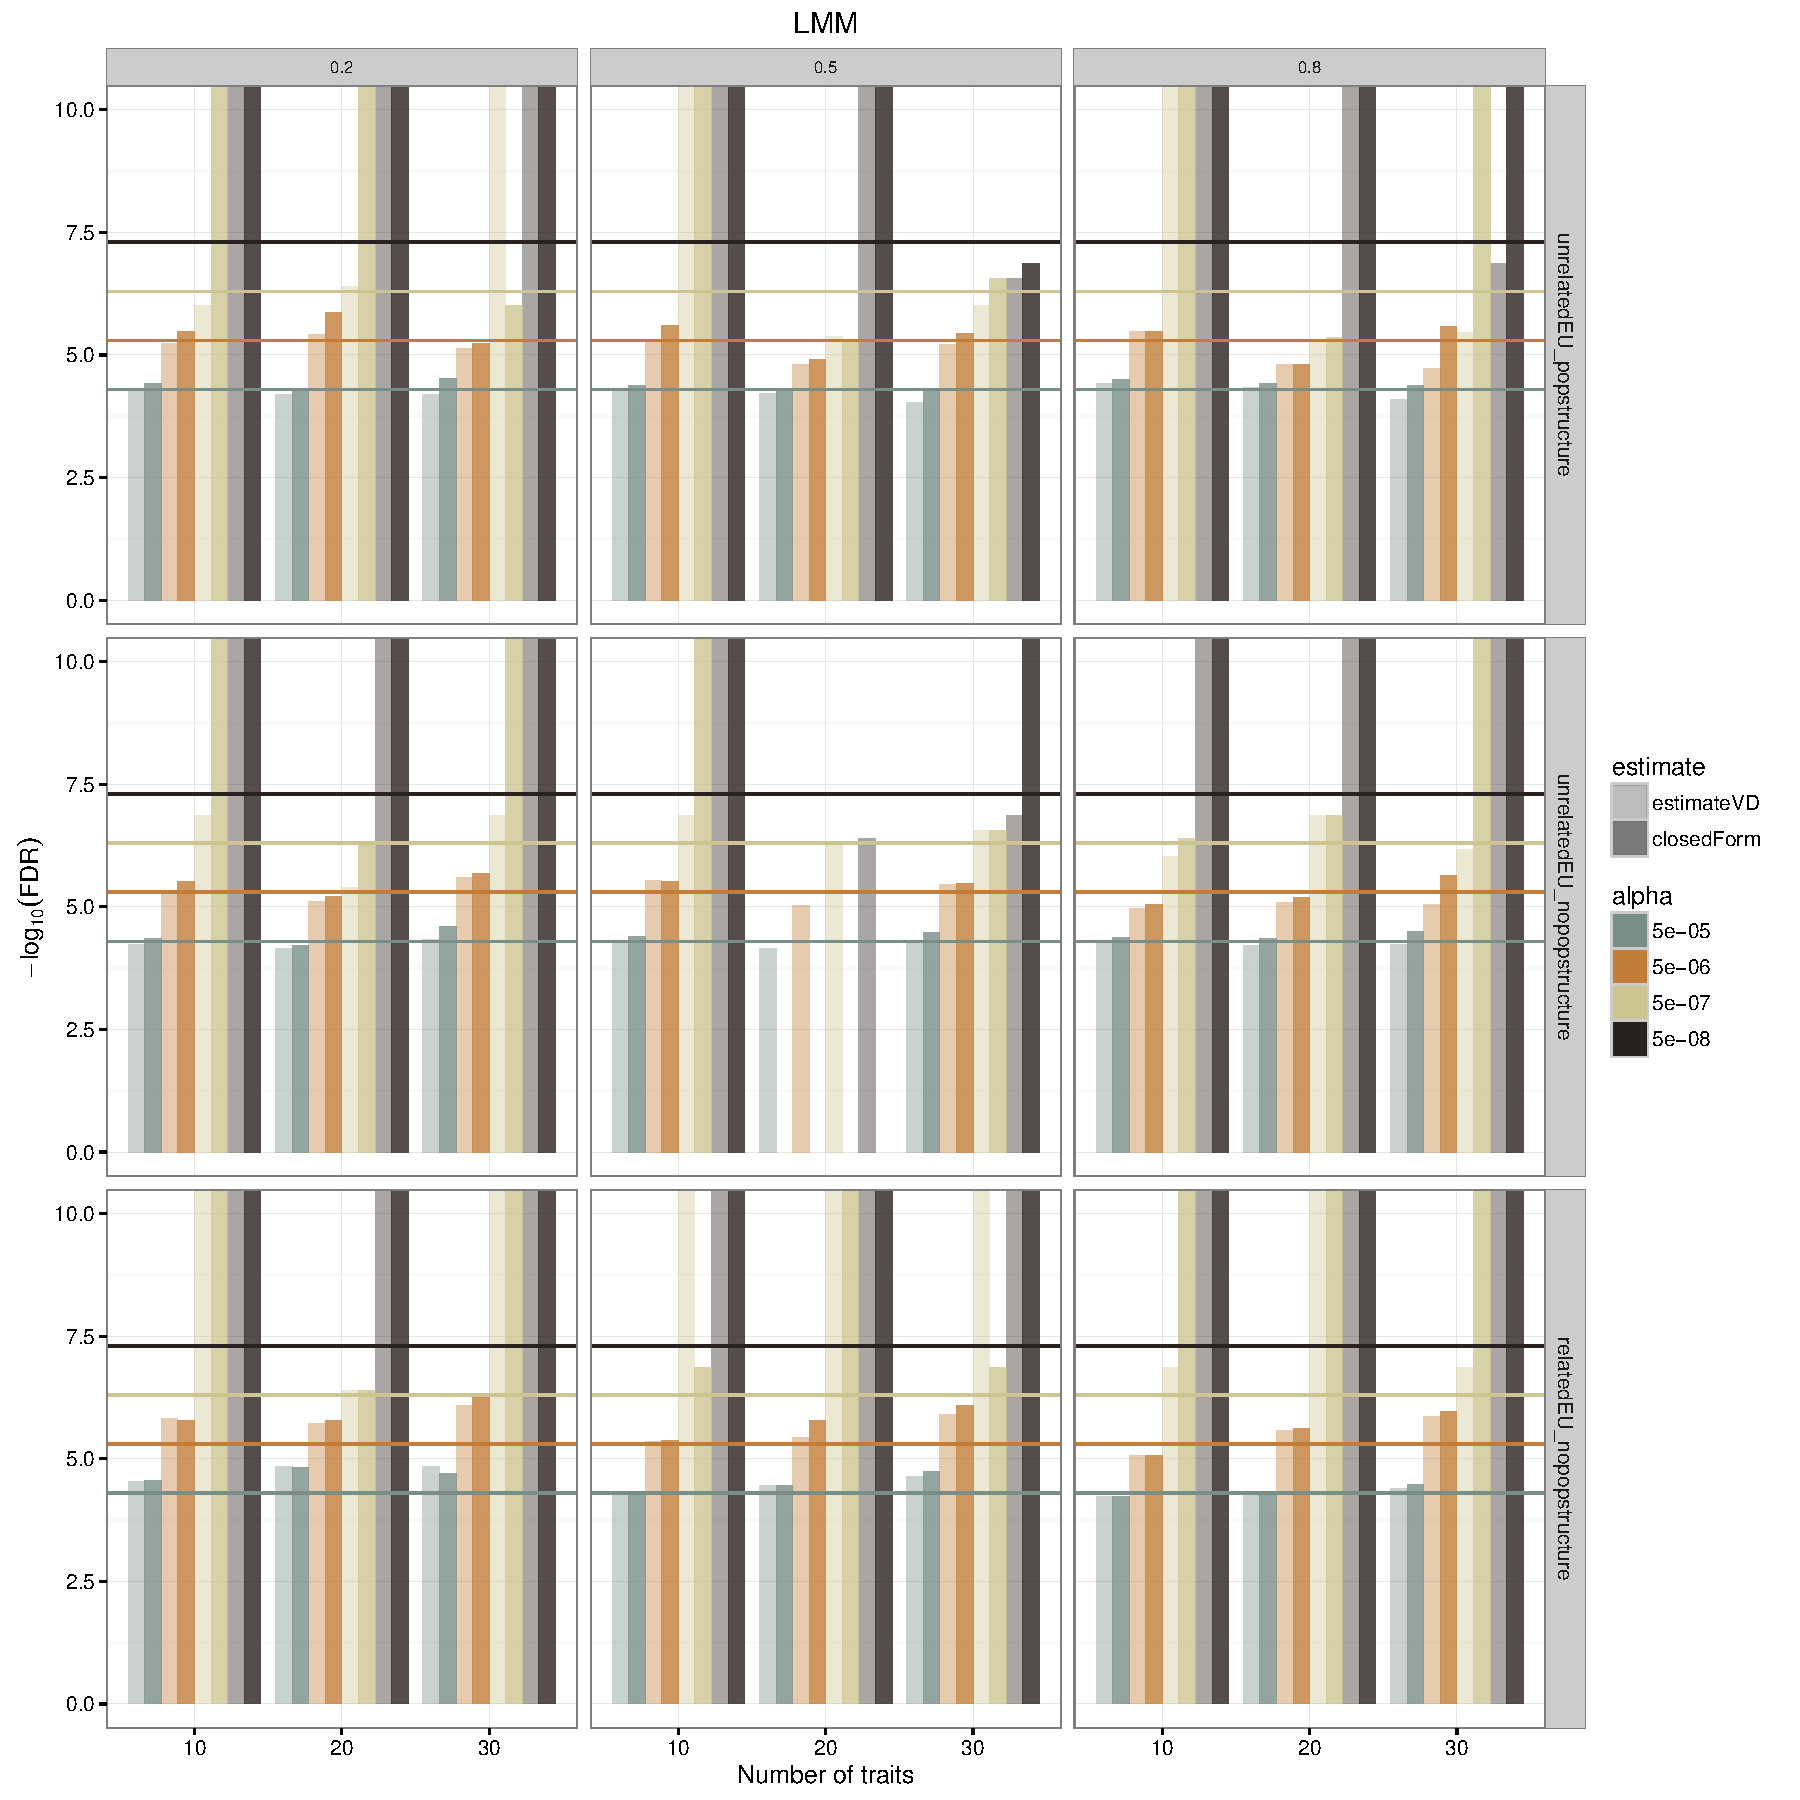
\includegraphics[trim = 0mm 0mm 0mm 0mm, clip, width=0.5\textwidth]{Chapter1/Figures/20161205_calibrationBGOnly_closedForm.pdf}
	\caption[Comparison of LMM based on RLM trait-trait covariance estimates to LiMMBo-derived estimates]{\textbf{Comparison of LMM based on RLM trait-trait covariance estimates to LiMMBo-derived estimates.}  For each genetic architecture (unrelatedEU\_popstructure, unrelatedEU\_nopopstructure, relatedEU\_nopopstructure) and percentage of variance explained by genetics (0.2, 0.5, 0.8; purely by background genetic effects), three different trait set sizes (10, 20, 30) were simulated and the calibration of the model was assesed by mtGWAS with LiMMBo-derived (estimateVD) RLM estimates (closedForm) of \(C_g\) and \(C_n\). For calibrated models, the FDR (depicted as bar charts in different transparency for both estimates) reaches as far or beyond the vertical line for the applied \(\alpha\) threshold. Overall, estimates from both models yield equally well calibrated results.}
 	\label{fig:closedForm}
\end{figure}

 
 \section{Model choice for mtGWAS depends on relatedness and population structure}
 \label{section:modelchoice}
Figure~\ref{fig:modelchoice} shows the calibration of the mtGWAS for either the LM with the first ten principle components (LM-PC) of the kinship matrix as covariates \(F\) (Figure~\ref{fig:calibration-lmpc}; Equation~\ref{eq:lm-mv}) or the LMM  (Figure~\ref{fig:calibration-lmm}; Equation~\ref{eq:lmm-mv}). The model calibration strongly depends on the underlying genetic architecture of the cohort. In cohorts without relatedness and structure,  LM-PC is much better calibrated than the LMM, whereas the LMM outperforms the LM-PC in cohorts with related individuals.

\begin{figure}[!h]
	\centering
	\begin{subfigure}[b]{0.45\textwidth}
		%\hspace{3cm}
		\center
	\includegraphics[page=2, trim = 0mm 0mm 28mm 5mm, clip, scale=0.25]{Chapter1/Figures/20170105_calibrationBGOnly.pdf}
	\caption{\textbf{Linear model with PCs}}
 		\label{fig:calibration-lmpc}
	\end{subfigure}
	~
	\begin{subfigure}[b]{0.45\textwidth}
		%\hspace{3cm}
		\center
	\includegraphics[page=3, trim = 0mm 0mm 0mm 5mm, clip, scale=0.25]{Chapter1/Figures/20170105_calibrationBGOnly.pdf}\\
	\caption{\textbf{Linear mixed model}}
 		\label{fig:calibration-lmm}
	\end{subfigure}
	\caption[Calibration of different models depending on population structure, number of traits and percentage of genetic variance]{\textbf{Calibration of different models depending on population structure, number of traits and percentage of genetic variance.} (a) The LM set-up is reasonably well-calibrated for populations of unrelated individuals (upper two panels) across all trait sizes but is no calibrated for populations wtih high inter-individual relatedness especially in cases with a strong underlying genetic cause of the trait. (b) The LMM is well-calibrated up to trait set sizes of 30-40 traits for unrelated populations, but loses calibration for larger trait set sizes (upper two panels). It stays well calibrated across all trait sizes for populations with related individuals (lower panel).}
 	\label{fig:modelchoice}
\end{figure}

